\documentclass[aspectratio=169,t,xcolor=table]{beamer}
\usepackage[utf8]{inputenc}

\usepackage{booktabs} 
\usepackage{subcaption}

\usetheme{Ufg}
% remove caption Fig 
\usepackage{caption}
\captionsetup{labelformat=empty,labelsep=none}


\usepackage{pgfpages}
\setbeameroption{show notes}
\setbeameroption{show notes on second screen}

% link to video player
\usepackage{multimedia}

%tikz figures
\usepackage{tikzit}
\input{figs/dodstyle.tikzstyles}
%-------------------------------------theorems--------------
\newtheorem{conj}{Conjetura}
\newtheorem{defi}{Definição}
\newtheorem{teo}{Teorema}
\newtheorem{lema}{Lema}
\newtheorem{prop}{Proposição}
\newtheorem{cor}{Corolário}
\newtheorem{ex}{Exemplo}
\newtheorem{exer}{Exercício}

\setbeamertemplate{theorems}[numbered]
\setbeamertemplate{caption}[numbered]

%-------------------------------------------------------------%
%----------------------- Primary Definitions -----------------%

% This command set the default Color, is also possible to choose a custom color
\setPrimaryColor{orange} 

% First one is logo in title slide (we recommend use a horizontal image), and second one is the logo used in the remaining slides (we recommend use a square image)
    \setLogos{lib/logos/matfyz.png}{lib/logos/matfyz.png} 


% -------------------------------------- Title Slide Information
\begin{document}
\title[Inf UFG]{(Adversarial) Multi-Agent Path Finding}
%\subtitle{Template Latex}

\author{Marika Ivanová}

\institute[UFG] % (optional)
{
  \inst~
  Department of Theoretical Computer Science and Mathematical Logic\\
  ~\newline
  Charles University in Prague \\
  Faculty of Mathematics and Physics
  ~\newline
  ~\newline
  ivanova@ktiml.mff.cuni.cz

}
%-----------------------The next statement creates the title page.
\frame[noframenumbering]{
	\titlepage

	\note{
		Hello and welcome to open day at Faculty of Mathematics and Physics.
		In this video we are going to talk about Adversarial Multi-Agent Path Finding, which is a topic in the area of Artificial Intelligence.
		First we will talk about traditional Multi-Agent Path Finding and then we show how to extend this problem by an adversarial element.
	}

}


%------------------------------------------------Slide 1
%\setLayout{vertical} % This command define the layout. 'vertical' can be replace with 'horizontal', 'blank, 'mainpoint', 'titlepage'
%
%\begin{frame}
%    \frametitle{Table of Contents}
%    \tableofcontents
%\end{frame}
%---------------------------------------------------------


%---------------------------------------------------------Slide 2
\section{Multi-Agent Path Finding}

\setLayout{horizontal}
\begin{frame}
    \frametitle{Multi-Agent Path Finding}
    \textbf{Problem description}
    \begin{itemize}
	    \item A group of agents (robots) deployed in a given environment
        \item Each agent has a defined initial and target location
        \item \textbf{Task:} relocate the agents to their targets while avoiding collisions
    \end{itemize}
    ~\newline
    \textbf{Objective function:}
    \begin{itemize}
        \item Minimum makespan
        \item Minimum total distance
        \item Minimum total arrival time
    \end{itemize}

	\note{

		Let us consider a group of agents, for example robots deployed in a given environment with obstacles.
		Each agent has a defined initial and target location.
		Our task is to navigate the agents to their respective target positions, so that they do not collide with each other or with the obstacles.

		We would also like to do it as best as possible.
		There are several criteria for assessing quality of a solution.
		The most common is to use so called minimum makespan, in which minimizes the time of the last arriving agent.
		There is also a possibility to minimize the total number of moves, which means that the agents should cover the shortest possible distance.
		Another option is to minimize total time that agents spend on their way.
	}
	
\end{frame}

%---------------------------------------------------------Slide 3
\setLayout{vertical}
\begin{frame}
\frametitle{Motivation}
\begin{columns}
\begin{column}{.5\textwidth}
\begin{itemize}
    \item Moving goods in warehouses
    \item Manipulation of shipping containers
    \item Navigation of a group of autonomous vehicles
\end{itemize}
\begin{figure}
        \centering
        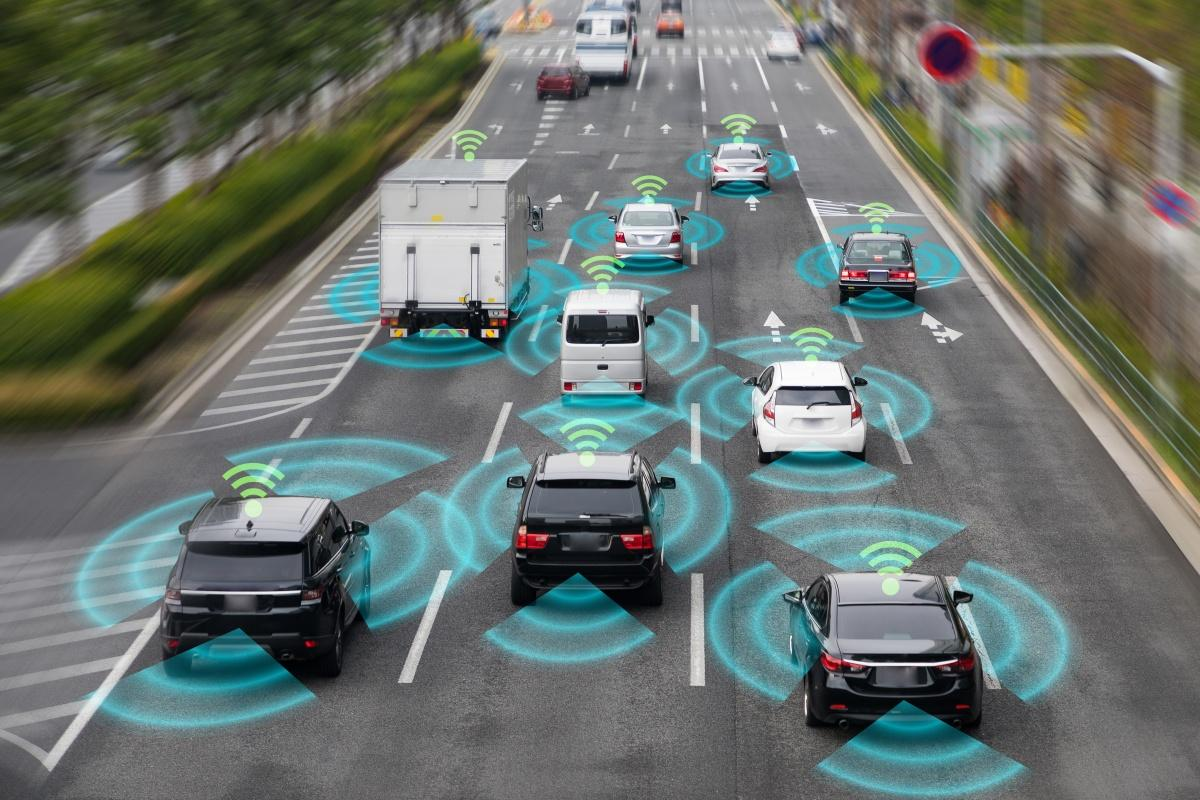
\includegraphics[width=.7\textwidth]{figs/autonomous-car.jpg}
    \end{figure}
 
\end{column}
\begin{column}{.4\textwidth}
    \begin{figure}
        \centering
        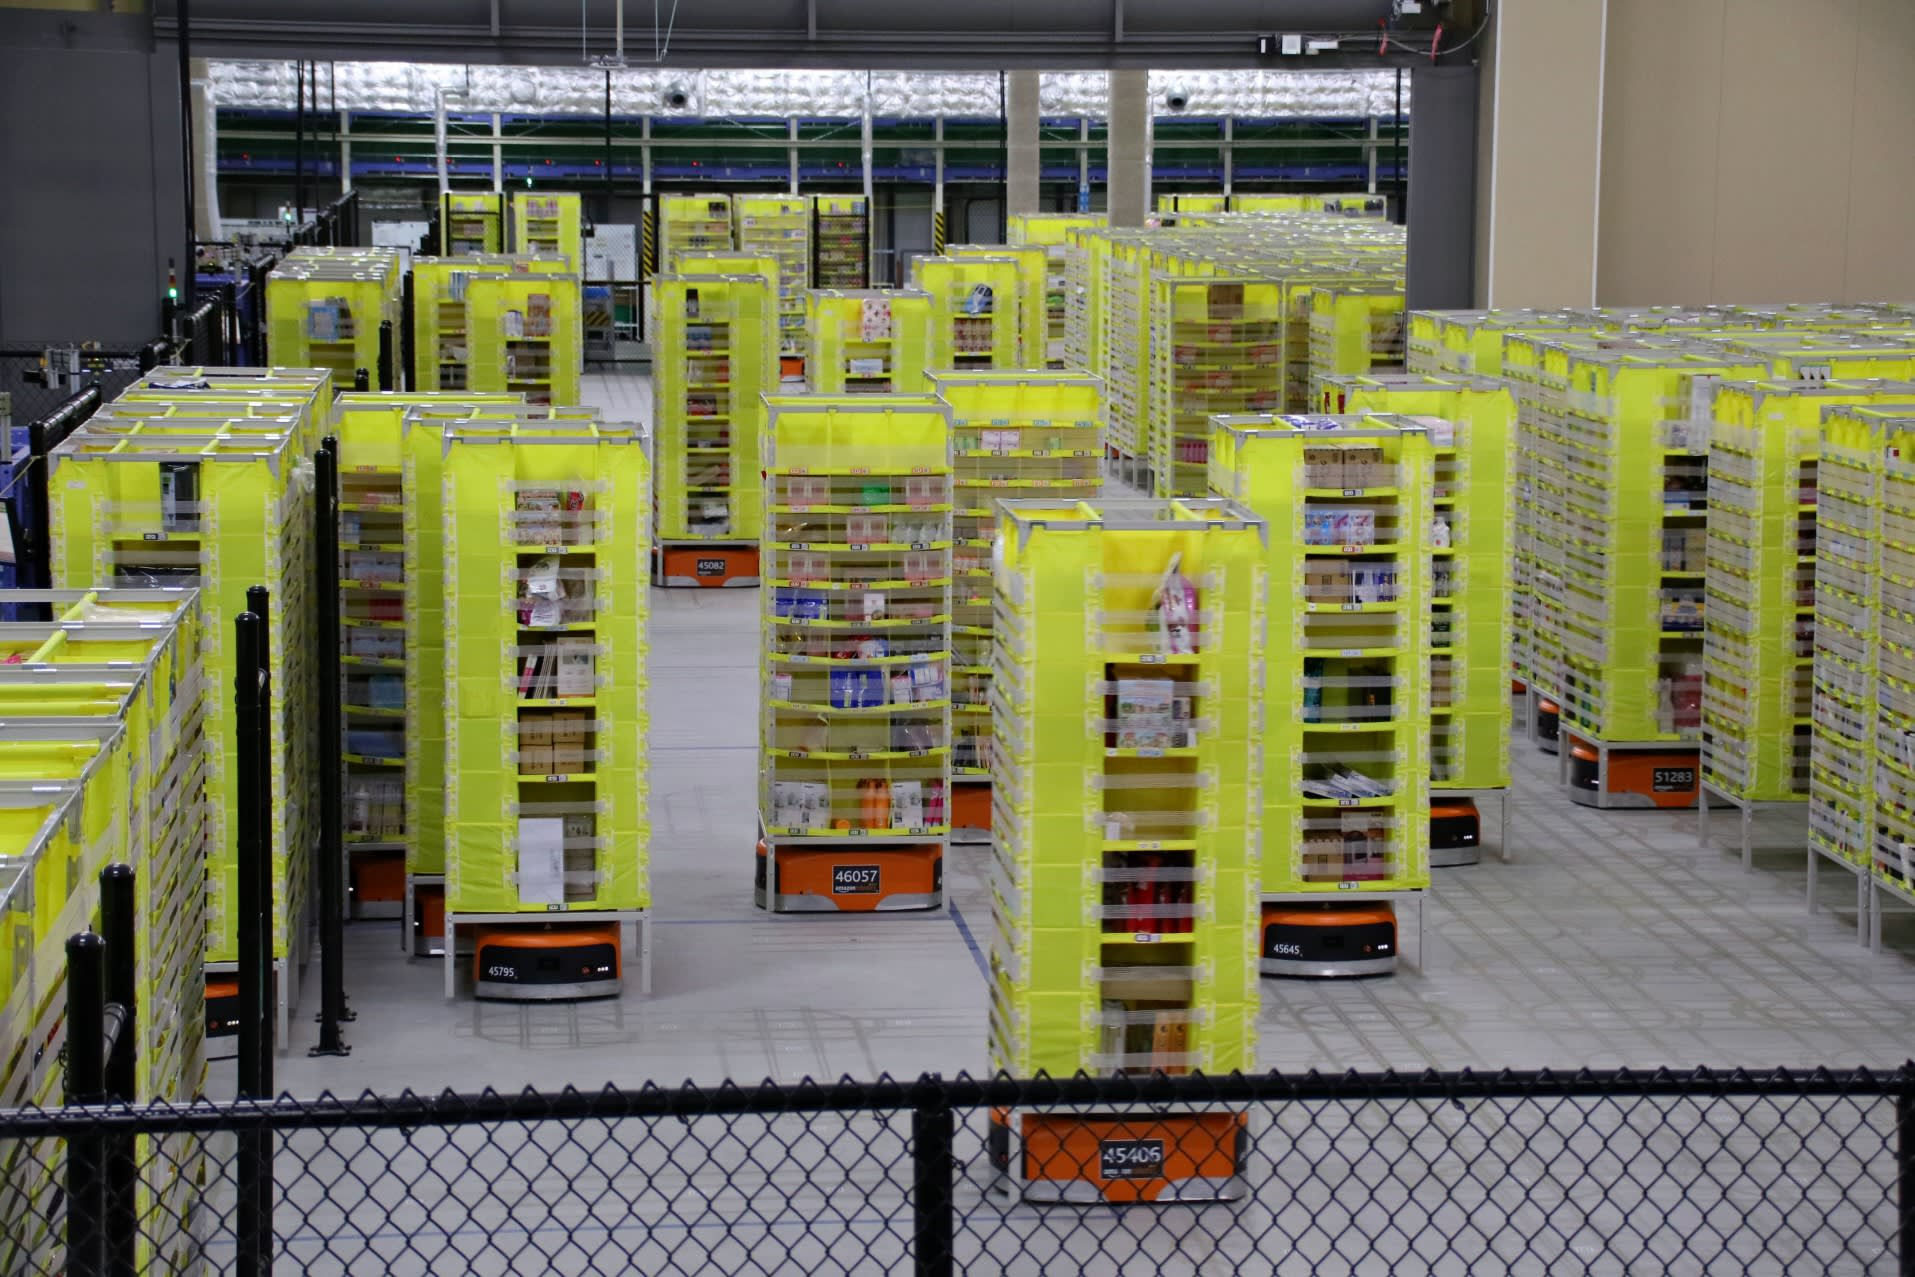
\includegraphics[width=.7\textwidth]{figs/roboti-amazon.jpg}
    \end{figure}
    
     \begin{figure}
        \centering
        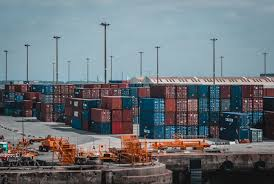
\includegraphics[width=.7\textwidth]{figs/shipping.jpg}
    \end{figure}
\end{column}
\begin{column}{.1\textwidth}
~
\end{column}
\end{columns}
	\note{

		This problem is motivated by various practical applications.
		Recently, robots have been widely used in large warehouses, where they move goods or racks from one place to another.
		Another logistic application is moving shipping containers.
		In this case, agents are the containers.
		It is clear that moving such large objects should be done as efficient as possible.
		Another hot topic is autonomous vehicle control, particularly in traffic jams.

	}

\end{frame}
\begin{frame}

\centering
\href{run:/usr/bin/xdg-open -fs vid/amazon.mp4}{
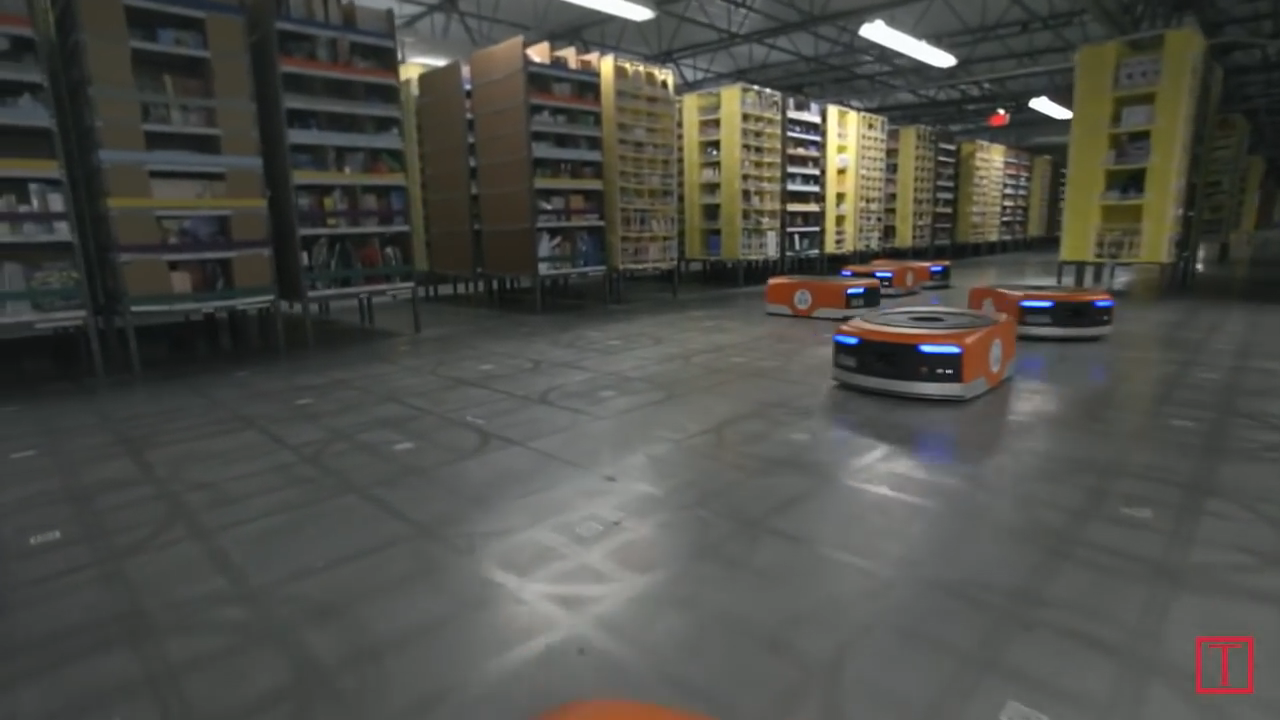
\includegraphics[scale=0.25]
{figs/amazon.png}}
\note{

	Here we have a short video showing how Kiwa robots move in Amazon warehouse.
	We can see a group of robots that need to relocate to a certain place and must not collide.
	}
\end{frame}
%---------------------------------------------------------Slide 3
\begin{frame}
\frametitle{Problem Abstraction}
\begin{columns}
\begin{column}{.4\textwidth}
    \begin{figure}
        \vspace{-20pt}
        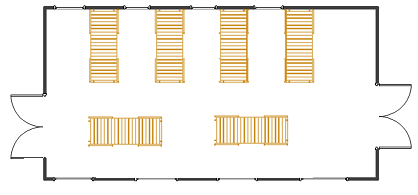
\includegraphics[width=1\textwidth]{figs/warehouse-plan-transp.png}
        %\caption{Template's Layouts.}
        %\label{fig:layouts}
    \end{figure}
    
     \begin{figure}
        \hspace{-10pt}
        \vspace{-30pt}
        \tikzfig{figs/warehouse-graph}
        %\caption{Template's Layouts.}
        %\label{fig:layouts}
    \end{figure}
\end{column}
\begin{column}{.6\textwidth}
\begin{itemize}
\item Mathematical formulation is necessary for theoretical study as well as processing by computer.
\item The environment is modeled by a graph
    \begin{itemize}
    \item Graph - set of vertices and edges
    \item Vertices - possible positions of agents
    \item Edges connect adjacent positions
    \end{itemize}
    \item Definition of initial and target locations
\end{itemize}

\end{column}

\end{columns}
	\note{

		In order to study the problem either theoretically or conduct simulations, it is necessary to define it formally.
		The environment in which agents are deployed is modeled by a graph.
		A graph is a mathematical structure consisting of a set of Vertices and a set of Edges.
		Vertices are points and edges are links between them.
		The vertices represent potential locations of agents, and the edges connect adjacent locations.
		Here in the figure above we can see a plan of some warehouse.
		We have one vertex for each positions in which a robot can stand 
		We assume that the robots can move in 4 directions, and so we obtain a grid graph like in the figure below.
	}
	
\end{frame}
%---------------------------------------------------------Slide 4
\begin{frame}
\frametitle{Movement Rules}
\begin{itemize}
    \item Each agent is located in one vertex
    \item Time divided into discrete time steps
    \item In each step an agent moves along an edge, or stays at its position 
    \item An agent can move to a vertex that is being left by another agent at the same time step
    \item Two agents cannot exchange their positions in one time step
\end{itemize}
\begin{columns}
    \begin{column}{.5\textwidth}
    \begin{figure}
        \centering
        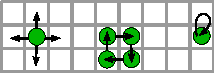
\includegraphics[width=.7\textwidth]{figs/moves.pdf}
        \end{figure}
    \end{column} 
    \begin{column}{.5\textwidth}
        \begin{figure}
        \centering
        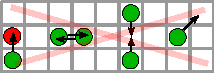
\includegraphics[width=.7\textwidth]{figs/nomovesx.pdf}
    \end{figure}
    \end{column}
\end{columns}
	\note{

		Next, it is necessary to define rules for agents' movement.
		Each agent is placed in exactly one vertex.
		Continuous time is divided into discrete time steps, for example seconds.
		In each time step an agent can move to an adjacent node along an edge, or stay at its position.
		An agent can also move to a vertex that is being left by another agent at the same time step.
		An exception to this rule is the case when two agents attempt to exchange their positions - that is not allowed.
		
	}
\end{frame}
%---------------------------------------------------------Slide 5
\setLayout{horizontal}
\begin{frame}
\frametitle{Multi-Agent Path Finding}
\begin{columns}
\begin{column}{.5\textwidth}
    \begin{figure}
    \begin{overprint} 
        \onslide<1>\tikzfig{figs/mapfex-makespan-1}
        \onslide<2>\tikzfig{figs/mapfex-makespan-2}
        \onslide<3>\tikzfig{figs/mapfex-makespan-3}
        \onslide<4->\tikzfig{figs/mapfex-makespan-4}
    \end{overprint} 
    \end{figure}
    
\end{column}
\begin{column}{.5\textwidth}
    \begin{figure}
    \begin{overprint} 
        \onslide<5>\tikzfig{figs/mapfex-sum-1}
        \onslide<6>\tikzfig{figs/mapfex-sum-2}
        \onslide<7>\tikzfig{figs/mapfex-sum-3}
        \onslide<8>\tikzfig{figs/mapfex-sum-4}
        \onslide<9>\tikzfig{figs/mapfex-sum-5}
    \end{overprint} 
    \end{figure}
    
\end{column}
\end{columns}
\begin{columns}
\begin{column}{.5\textwidth}
    \only<1>{
    \begin{itemize}
     \item[] makespan: \textcolor{red}{0} 
     \item[] sum-of-costs: 0
    \end{itemize}
     }
    \only<2>{
        \begin{itemize}
        \item[] makespan: \textcolor{red}{1}
        \item[] sum-of-costs: 2
        \end{itemize}
    }
    \only<3>{
        \begin{itemize}
    \item[] makespan: \textcolor{red}{2}    
    \item[] sum-of-costs: 4
        \end{itemize}
    }
    \only<4->{
        \begin{itemize}
    \item[] makespan: \textcolor{red}{3} 
    \item[] sum-of-costs: 6
        \end{itemize}
    }
\end{column}
\begin{column}{.5\textwidth}
    \only<5>{
        \begin{itemize}
    \item[] makespan: \textcolor{red}{0} 
    \item[] sum-of-costs: 0
        \end{itemize}
    }
    \only<6>{
        \begin{itemize}
    \item[] makespan: \textcolor{red}{1} 
    \item[] sum-of-costs: 2
        \end{itemize}
    }
    \only<7>{
        \begin{itemize}
    \item[] makespan: \textcolor{red}{2}    
    \item[] sum-of-costs: 3
        \end{itemize}
    }
    \only<8>{
        \begin{itemize}
    \item[] makespan: \textcolor{red}{3} 
    \item[] sum-of-costs: 4
        \end{itemize}
    }
    \only<9->{
        \begin{itemize}
    \item[] makespan: \textcolor{red}{4} 
    \item[] sum-of-costs: 5
        \end{itemize}
    }
\end{column}
\end{columns}
	\note{	

		Now we will see an example of a simple instance with two agents.
		The Vertices in green circles are targets of the agents.
		We will see what is the optimal solution for the shortest arrival time of the last agent, called minimum makespan.
		Although a2 stands right next to its target, it will not move there in the first step.
		Instead of that, A1 rushes via the shortest path towards its target.
		A2 thus gives way to A1
		When A1 is performing the last move A2 can simultaneously  move to its target.
		This solution has makespan 3, while total arrival time of all agents is 6.

		Now we will see a solution with a longer makespan, but shorter total arrival time.
		In this solution A2 immediately moves to its target, and A1 has to go along the longer upper path.
		This solution has total arrival time 5, which is optimal.
		On the other hand, makespan is 4, which can be done better as we have seen in the previous example.


	}
\end{frame}
%---------------------------------------------------------Slide 5
\begin{frame}
\frametitle{Solution methods}
\begin{enumerate}
    \item<1-> Centralized
        \begin{itemize}
        \item<2-> Agents regarded as one entity
        \item<2-> Paths are searched simultaneously
        \end{itemize}
        \vspace{20pt}
	\item<1-> Decentralized (decoupled)
        \begin{itemize}
        \item<3-> Agents processed individually 
        \end{itemize}
	\item[]<4-> Centralized methods typically yield a better solution, but are computationally more challenging
\end{enumerate}
	\note{	

		Solution methods are divided into two main groups - centralized and decentralized.
		In centralized approaches, whole group of agents is considered as a single entity.
		Paths are then searched simultaneously for all agents.
		In centralized methods are paths searched individually for each agent.
		Centralized methods typically yield a better solution than decentralized methods, however, centralize approaches are often computationally more challenging.
	}

\end{frame}

%---------------------------------------------------------Slide 6
\setLayout{vertical}
\begin{frame}
\frametitle{\\\textcolor{orange}{Adversarial} Multi-Agent Path Finding (AMAPF)}
\begin{columns}
\begin{column}{.65\textwidth}
\begin{itemize}
    \item Generalization of MAPF
    \item Agents divided into two competing teams
    \begin{itemize}
        \item<2-> \textcolor{orange}{Attackers $A$} 
        \item<2-> \textcolor{orange}{Defenders $D$} 
    \end{itemize}
        \item<3-> Attackers aim to reach their target positions
        \item<3-> Defenders protect the targets from attackers
    \item<4-> Two player game
    \item<4-> Teams take turns in each step
    \item<5-> \textbf{Motivation: } military and security simulations, video game industry
\end{itemize}
\end{column}
\begin{column}{.35\textwidth}
        \begin{figure}
        \hspace{-60pt}
        \vspace{-40pt}
        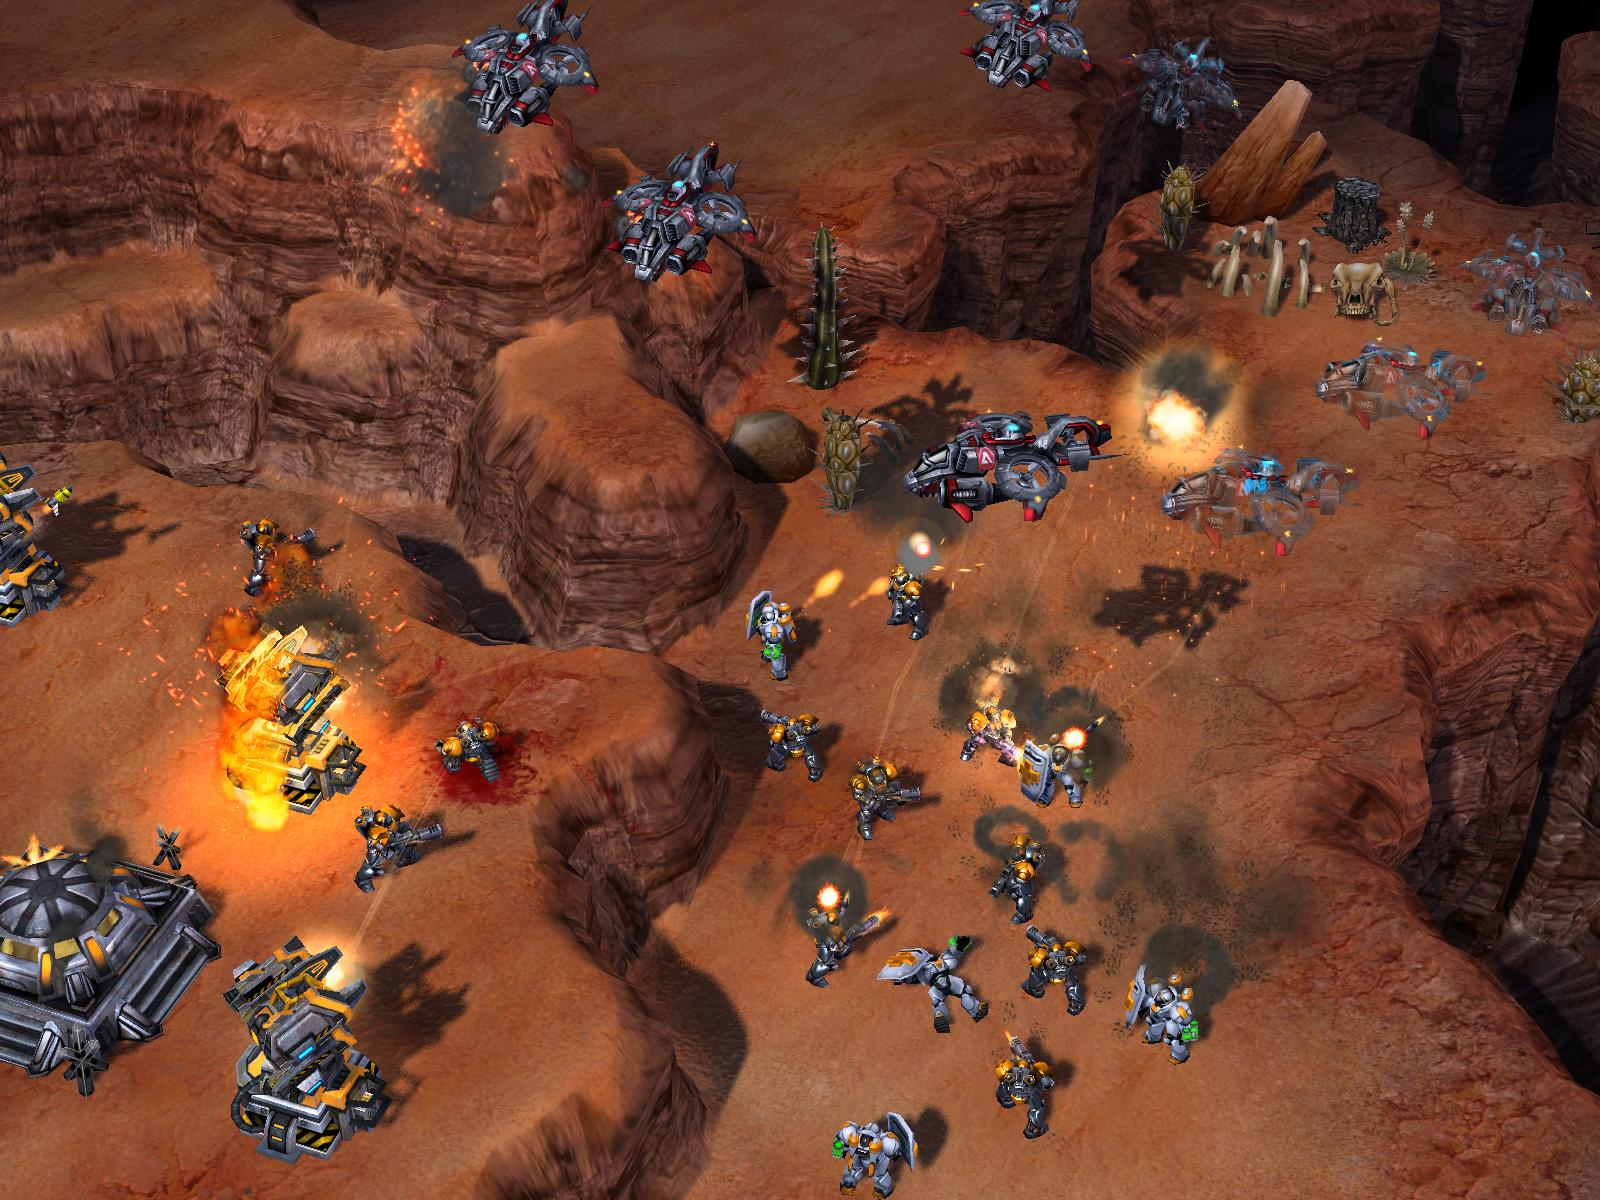
\includegraphics[width=.8\textwidth]{figs/game.jpg}
    \end{figure}
\end{column}
\end{columns}
	\note{	

		A generalization of the problem introduces an adversarial element in multi agent path finding.
		Agents are divided into two competing teams called Attackers and defenders.
		Attackers' task is the same as we have seen so far: they need to navigate agents to their target positions while avoiding collisions.
		Defenders on the other hand try to protect these targets from the attackers.
		The problem becomes a two player games where teams as players take turns.
	}
\end{frame}
%---------------------------------------------------------Slide 7
\begin{frame}
\frametitle{\textcolor{orange}{Adversarial} Multi-Agent Path Finding (AMAPF)}
\begin{itemize}
    \item[]<1-> \textbf{Victory of attackers:} all agents from $A$ reach their targets
    \item[]<1-> \textbf{Problem:} find a winning strategy for $A$
\end{itemize}
\begin{block}<2->
{Winning strategy}
In each step which is $A$'s turn, $A$ plays such a move that leads to its victory regardless of the response of defenders $D$.
\end{block}
\vspace{20pt}
\begin{itemize}
	\item<3-> The decision whether there exists a winning strategy is very hard \\ (\textcolor{orange}{PSPACE-hard})
	\item<4-> It is probably even harder (\textcolor{orange}{EXPTIME-hard})
\item<5-> You will get to know what that means when you join us :)
\end{itemize}
	\note{	

		The team of attackers wins in case all its agents manage to arrive at their targets.
		Our task is to find a winning strategy for the team of attackers.
		A winning strategy means that in each step when attacker is to move, they play such a move that defenders cannot prevent victory of attackers no matter how they play.
		Theoretical study of this problem shows that already the decision whether a winning strategy for attackers exists is very hard, specifically PSPACE-hard.
		Recently, it seems however that it is even harder, which we call EXPTIME hard
		You will find out more about these strange terms when you come to study at our faculty.

	}

\end{frame}

\begin{frame}
	\frametitle{Demonstration of agents' movement in an AMAPF instance}
	\note{

		Now we will have a look at a short visualisation of movement of agents in Adversarial multi agent path finding.
		Three light green attackers 4 5 and 6 at the top has three dark green targets at the bottom.
		Agent 3 has its target in the remaining dark green node.
		Let us have a look at what movement the green attackers have to perform, so that the red defenders would not prevent them from reaching the targets.

	}
\end{frame}
%---------------------------------------------------------Slide 8
\setLayout{horizontal}
\begin{frame}
\frametitle{Solution methods}
	\begin{itemize}
		\item In a typical instance, not all attackers manage to reach their target
		\item We therefore focus on occupying as many targets as possible
	\end{itemize}
\begin{columns}
	\vspace{20pt}
\begin{column}{.33\textwidth}
\textbf{Greedy}\newline

		The move that seems the most promising in a current situation is performed. 
		Assessed according to various criteria.
\end{column}
\begin{column}{.33\textwidth}
\textbf{Game}\newline

		Classic (alpha-beta) as well as less known (Monte Carlo tree search) used in two player games such as chess and go
\end{column}
\begin{column}{.33\textwidth}
\textbf{MAPF}\newline

		Adaptation of methods designed for MAPF 
\end{column}
\end{columns}
    	\note{	

		In the majority of instances it is not possible that all attackers reach their targets.
		We therefore try to maximize the number of targets captured by attackers.
		We propose algorithms that get some instance as an input, and whenever it is attacker's turn, it selects its move.
		So far we have evaluated three types of algorithms
		The simplest greedy methods perform the move that seems to lead tho the best position.
		This can often be a bit myopic.
		On the other hand, game algorithms such as minimax alpha beta and others try to look a bit further ahead,
		and perform such a move that leads to the best possible result in a certain time frame.
		There are many approaches designed For traditional multi agent path finding
		It is also possible to adapt them so that they contain the adversarial element.
	}

\end{frame}
%--------------------------------------------------------- Slite 9
\begin{frame}
\frametitle{Future research}
\begin{itemize}
    \item[] MAPF has been studied extensively since last several years
    \item[] That is not the case for AMAPF
    \item[] 
    \item[] Possible directions of future research:
    
        \begin{itemize}
        \item Computational complexity of special cases
        \item More detailed evaluation of solution techniques
        \item Design of new solution methods
        \item Strategy for the team of defenders
	\item Study of modified problems (e.g., not all agents have targets)
        \end{itemize}
\end{itemize}
	\note{	
		Adversarial Multi agent path finding is a topic with a good research potential
		It can be studied both theoretically and practically, and interesting results  are awaited  in both directions.
		The results are expected to be published on international conferences on artificial intelligence and related topics.

		}
\end{frame}
\begin{frame}
	\frametitle{Sources}
	\begin{enumerate}
		\item Adversarial Cooperative Path-Finding: Complexity and Algorithms, 2014 IEEE 26th International Conference on Tools with Artificial Intelligence
		\item Adversarial Cooperative Path-Finding: A First View, AAAI (Late-Breaking Developments) 2013
		\item www.koupy.net/graphrec.php
		\item www.therobotreport.com
		\item www.smartcitiesworld.net
	\end{enumerate}
	\note{

		So this was a short presentation about adversarial multi agent path finding, thank you very much for watching.

	}

\end{frame}


\end{document}
